\documentclass[14pt]{extarticle}
\usepackage{amsmath}
\usepackage{amssymb}
\usepackage{tikz}
\usetikzlibrary{calc}
%\usetikzlibrary{trees}
\usepackage{hyperref}
\usepackage{graphicx}
\graphicspath{ {../../chap05/} }
\usepackage[top=0.75in, bottom=0.75in, left=0.75in, right=0.75in]{geometry}
\newcommand*{\Scale}[2][4]{\scalebox{#1}{\ensuremath{#2}}}%
\usepackage[shortlabels]{enumitem}
\usepackage[most]{tcolorbox}
\definecolor{bg}{RGB}{255,249,227}
% \usepackage{showframe}
\title{\vspace{-5ex}Math 208 Section 5.1}
\date{\vspace{-10ex}}
\usepackage{multicol}
\setlength{\columnsep}{1cm}
\newcommand{\tikzmark}[1]{\tikz[overlay,remember picture] \node (#1) {};}
\newcommand{\DrawBox}[4][]{%
	\tikz[overlay,remember picture]{%
		\coordinate (TopLeft)     at ($(#2)+(-0.2em,0.9em)$);
		\coordinate (BottomRight) at ($(#3)+(0.2em,-0.3em)$);
		%
		\path (TopLeft); \pgfgetlastxy{\XCoord}{\IgnoreCoord};
		\path (BottomRight); \pgfgetlastxy{\IgnoreCoord}{\YCoord};
		\coordinate (LabelPoint) at ($(\XCoord,\YCoord)!0.5!(BottomRight)$);
		%
		\draw [red,#1] (TopLeft) rectangle (BottomRight);
		\node [below, #1, fill=none, fill opacity=1] at (LabelPoint) {#4};
	}
}

\begin{document}
\maketitle		
\section*{Homework, Reading, and Other}
\begin{itemize}
	\item Exam 1
	\item Section 5.1
\end{itemize}

\section*{Goals}
\begin{itemize}
	\item Understand, manipulate, and graph linear inequalities.
	\item From a graph, determine the linear inequality.
\end{itemize}

\section*{5.1 Linear Inequalities in two Variables}
A \textit{Linear Inequality} is similar to a linear equation but instead of the '=',  we use an inequality operator, i.e: $ <, \leq , >, \geq$. On a number line and with one variable this is easy to understand, such as $ 3<7$ or $x \geq -5$. In this chapter, we work with two variables and show the solutions using a graph.

\subsection{Graphing Linear Inequalities}
See these \href{https://www.desmos.com/calculator/fyoyd1n4op}{Desmos graphs}
\\\\
Start with the equation to the line $y = x-2$. This equation divides the plane into upper/lower or left/right halves. From this equation, we can demonstrate four inequalities. A dashed line indicates the inequality is strictly greater than or strictly less than while a solid line allows equality.
\\\\
Sometimes it is obvious which part of the graph to shade but often it is not obvious. There is a simple method that allows for correctly determining the shaded region.

\begin{tcolorbox}[enhanced jigsaw,colback=bg,boxrule=0pt,arc=0pt]
	\textbf{Procedure to Graph Linear Inequalities}\\
	for $Ax + By$ $\square$ $C$.
	\begin{enumerate}
		\item Find any two points on the line  $Ax + By = C$. The x and y intercepts are good choices.
		\item Graph Ax + By = C as a dashed line if equality is not included in the original statement, or as a solid line if equality is included.
		\item Choose a test point anywhere in the plane not on the line and substitute the coordinates into the inequality. The origin, $(0, 0)$, usually requires the least computation.
		\item If the inequality gives a true statement, shade the half-plane that contains the test point. If not, shade the opposite half-plane.
	\end{enumerate}
\end{tcolorbox}


\subsection{Examples}
\subsubsection*{Graph $2x – 5y \leq 10$}
\begin{enumerate}
	\item $2x – 5y = 10$ \\ then 
	\begin{tabular}{c|c}
		x & y \\
		\hline
		0 & -2 \\
		5 & 0 \\
	\end{tabular}
	\item Equality is included so solid line
	\item Use $(0,0)$ as test point. Then 
	\begin{align*}
		2*0 -5*0 &\leq 10 \\
		0 &\leq 10
	\end{align*}
	\item Since $0 \leq 10$ is true, shade the half-plane that contains $(0,0)$.
\end{enumerate}
\begin{center}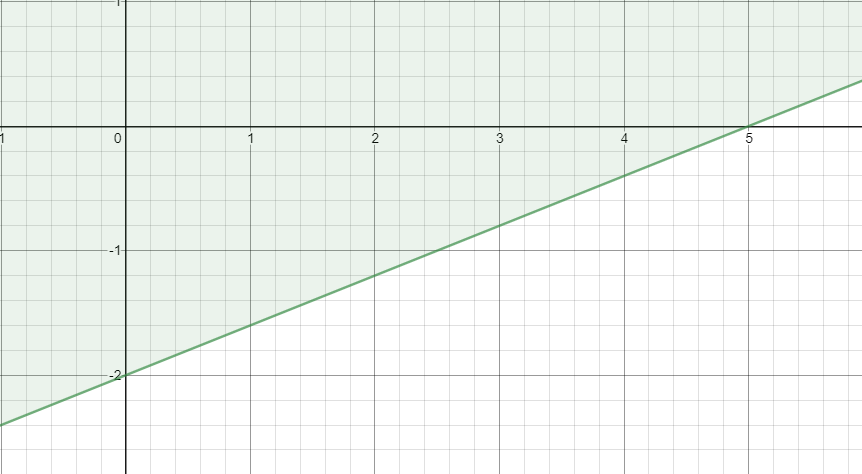
\includegraphics[width=0.5\linewidth]{5-1-1}\end{center}

\subsubsection*{Graph $–y < \frac{3}{2}x -3$}
First, use some algebra:
\begin{align*}
	–y &< \frac{3}{2}x -3 \\
	-\frac{3}{2}x - y &< -3
\end{align*}
When multiplying an inequality by a negative number, reverse the inequality.
\begin{align*}
	\frac{3}{2}x +y &>3 \\
	3x + 2y &>6
\end{align*}
\begin{enumerate}
	\item $3x + 2y =6$ \\ then 
	\begin{tabular}{c|c}
		x & y \\
		\hline
		0 & 3 \\
		2 & 0 \\
	\end{tabular}
	\item Equality is not included so dashed line
	\item Use $(0,0)$ as test point. Then 
	\begin{align*}
		3*0 + 2*0 &>6\\
		0 &> 6
	\end{align*}
	\item Since $0 >6$ is false, shade the half-plane that does not contain $(0,0)$.
\end{enumerate}
\begin{center}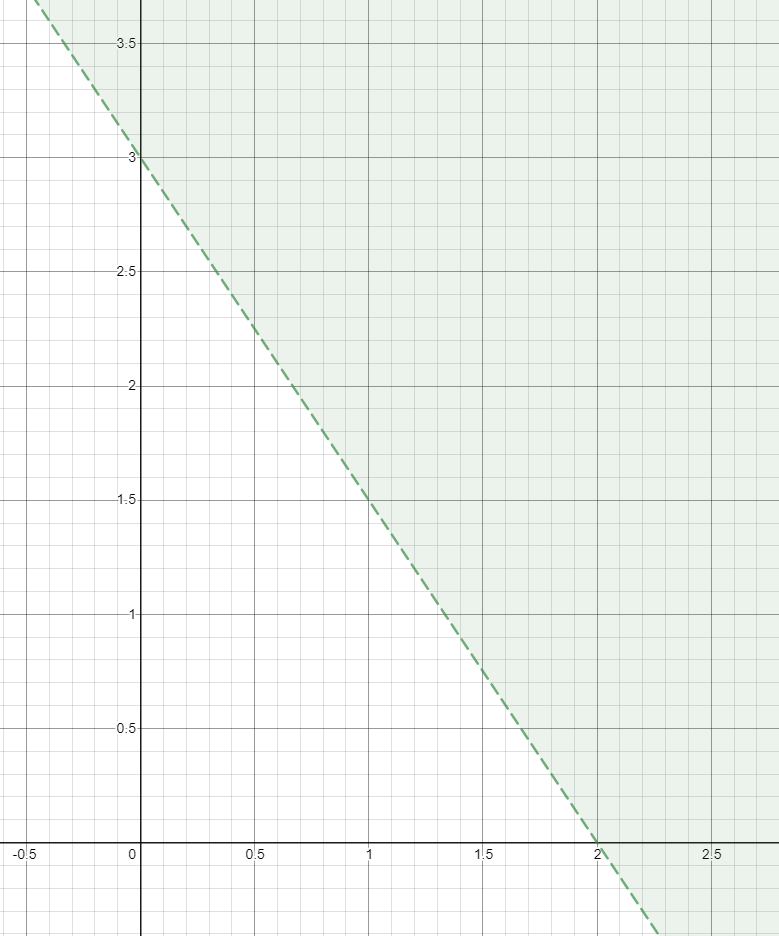
\includegraphics[width=0.5\linewidth]{5-1-2}\end{center}

\noindent\rule{\textwidth}{1pt}
{\footnotesize Copyright (C) 2021 Garold Dalton --- Released under GNU General Public License v3.0}


\cleardoublepage


\end{document}
